%label:"fig:symplecticDehnTwist"
%author:JeffHicks
%name:"symplectic Dehn twist"
%type:"figure"
%parent:"con:dehnTwist"
%caption:"Performing a Dehn twist on the zero section of $T^*S^1$"



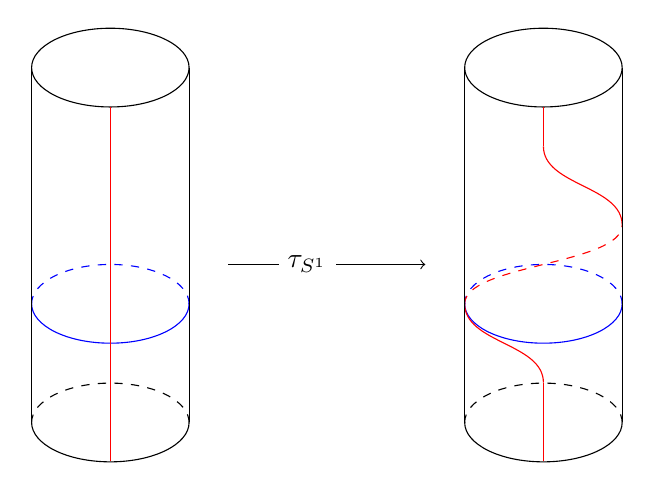
\begin{tikzpicture}

    \begin{scope}[]
    \draw  (-2.5,2.5) ellipse (1 and 0.5);
    
    \begin{scope}[shift={(0,-0.007)}]
    \begin{scope}[]
    
    \clip  (-1.45,-2.55) rectangle (-3.55,-2);
    \draw[]  (-2.5,-2) ellipse (1 and 0.5);
    
    \end{scope}
    \begin{scope}[]
    
    \clip  (-1.45,-1.45) rectangle (-3.55,-2);
    \draw[ dashed]  (-2.5,-2) ellipse (1 and 0.5);
    
    \end{scope}
    \end{scope}\begin{scope}[shift={(0,1.5)}]
    \begin{scope}[]
    
    \clip  (-1.45,-2.55) rectangle (-3.55,-2);
    \draw[blue]  (-2.5,-2) ellipse (1 and 0.5);
    
    \end{scope}
    \begin{scope}[]
    
    \clip  (-1.45,-1.45) rectangle (-3.55,-2);
    \draw[blue, dashed]  (-2.5,-2) ellipse (1 and 0.5);
    
    \end{scope}
    \end{scope}\begin{scope}[shift={(0,0.5)}]
    
    \draw[red] (-2.5,-2) .. controls (-2.5,-1.5) and (-3.5,-1.5) .. (-3.5,-1);
    \draw[red, dashed] (-3.5,-1) .. controls (-3.5,-0.5) and (-1.5,-0.5) .. (-1.5,0);
    \draw[red] (-1.5,0) .. controls (-1.5,0.5) and (-2.5,0.5) .. (-2.5,1);
    \draw[red] (-2.5,-3) -- (-2.5,-2) (-2.5,1) -- (-2.5,1.5);
    \end{scope}
    \draw (-3.5,2.5) -- (-3.5,-2);
    \draw (-1.5,2.5) -- (-1.5,-2);dig
    \end{scope}
    
    \begin{scope}[shift={(-5.5,0)}]
    \draw  (-2.5,2.5) ellipse (1 and 0.5);
    
    \begin{scope}[shift={(0,-0.007)}]
    \begin{scope}[]
    
    \clip  (-1.45,-2.55) rectangle (-3.55,-2);
    \draw[]  (-2.5,-2) ellipse (1 and 0.5);
    
    \end{scope}
    \begin{scope}[]
    
    \clip  (-1.45,-1.45) rectangle (-3.55,-2);
    \draw[ dashed]  (-2.5,-2) ellipse (1 and 0.5);
    
    \end{scope}
    \end{scope}\begin{scope}[shift={(0,1.5)}]
    \begin{scope}[]
    
    \clip  (-1.45,-2.55) rectangle (-3.55,-2);
    \draw[blue]  (-2.5,-2) ellipse (1 and 0.5);
    
    \end{scope}
    \begin{scope}[]
    
    \clip  (-1.45,-1.45) rectangle (-3.55,-2);
    \draw[blue, dashed]  (-2.5,-2) ellipse (1 and 0.5);
    
    \end{scope}
    \end{scope}
    \draw (-3.5,2.5) -- (-3.5,-2);
    \draw (-1.5,2.5) -- (-1.5,-2);
    \draw[red] (-2.5,2) -- (-2.5,-2.5);
    \end{scope}
    \draw[->] (-6.5,0) -- (-4,0);
    \node[fill=white] at (-5.5,0) {$\tau_{S^1}$};
    \end{tikzpicture}